\section{Automated plot generation (Stage 2)}
\label{sec:visualizer:plotgeneration}

\subsection{Decision tree classification of user interests}
\label{sec:visualizer:plotgeneration:tree}

Given initialization and actively selected labeled data, what classification 
models can the visualization system use to create a final fitted model of user 
interests? A \textbf{random forest} is such one model for classifying and 
labeling data 
(features of plots, in the case of the VS). In a random forest, various 
decision trees are constructed from random samples of the data. Each classifier 
has a vote of weight one for each unlabeled data, and the forest is aggregated 
by majority vote, which makes the resulting tree more accurate on average. The 
result is easily presented to the analyst in the form of a decision tree, which 
aids in user interpretability of the system output. A \textbf{decision tree} is 
a visual 
mapping of the sample space partitioning (decision boundaries). A simplistic 
example may be found in Figure~\ref{fig:visualizer:al:tree}. As such, the VS 
sets the choice of classification model to random forest by default but 
allows the user to specify their preferred classification model if they wish to 
do so.

\subsection{User interaction with active learning output}
\label{sec:visualizer:plotgeneration:user}

The system has now learned which of the unlabeled plots 
may be of interest to the user. The final learned classifier is used to fit the 
rest of the $d \choose 2$ unlabeled scatterplots, and a visual graph $G=(V,E)$ 
may be built from these labels with the following heuristic where $i,j \in 
\{1,...,d\}$:

\begin{algorithm}
	If label($i,j)>0$ (i.e. ``interesting'' instead of ``uninteresting''), draw 
	edge $E_{i,j}$
\end{algorithm}

Furthermore, the VS may provide a visualization of the resulting classifier 
itself such as the decision tree itself. The active learning output may be 
visualized as a heat map. A 
classic heat map represents each pair of variables as colors from a bivariate 
spectrum. Heat maps are difficult to interpret as it is one-dimensional; each 
end of the color spectrum represents minimum and maximum values respectively. 
It is unclear what the max or the min is as it depends on the domain of the 
whatever the heat map is plotting; as such, the minimum may not necessarily be 
negative while the maximum may not necessarily be positive. Furthermore, the 
subtle variations in hue between colors make it difficult to compare relative 
ranking among different pairs for colors that are similar. Buja \textit{et al.} 
propose an alternate, clearer method of visualizing the heat map, termed the 
``association navigator''~\cite{buja2016}. The association navigator is 
two-dimensional: the size of each color corresponds to its value while the 
color 
represents a positive or negative value~\cite{buja2016}. As such, the 
association navigator only utilizes two colors rather than a spectrum of 
colors, making it simple to distinguish between the two. By simplifying the 
color scheme and adding the dimension of size, the association navigator makes 
it much easier to interpret and compare different pairs of data at a glance. 
The stark difference between a traditional heatmap and the association 
navigator when applied to the same dataset may be seen in 
Figure~\ref{fig:visualizer:heatmap}. The VS provides both options, allowing the 
analyst to select whichever is easier to for them to interpret. 
With these visualizations of the active learning output, the user should be 
able to understand his/her own interests. 

\begin{figure}[htb]
	\begin{center}
		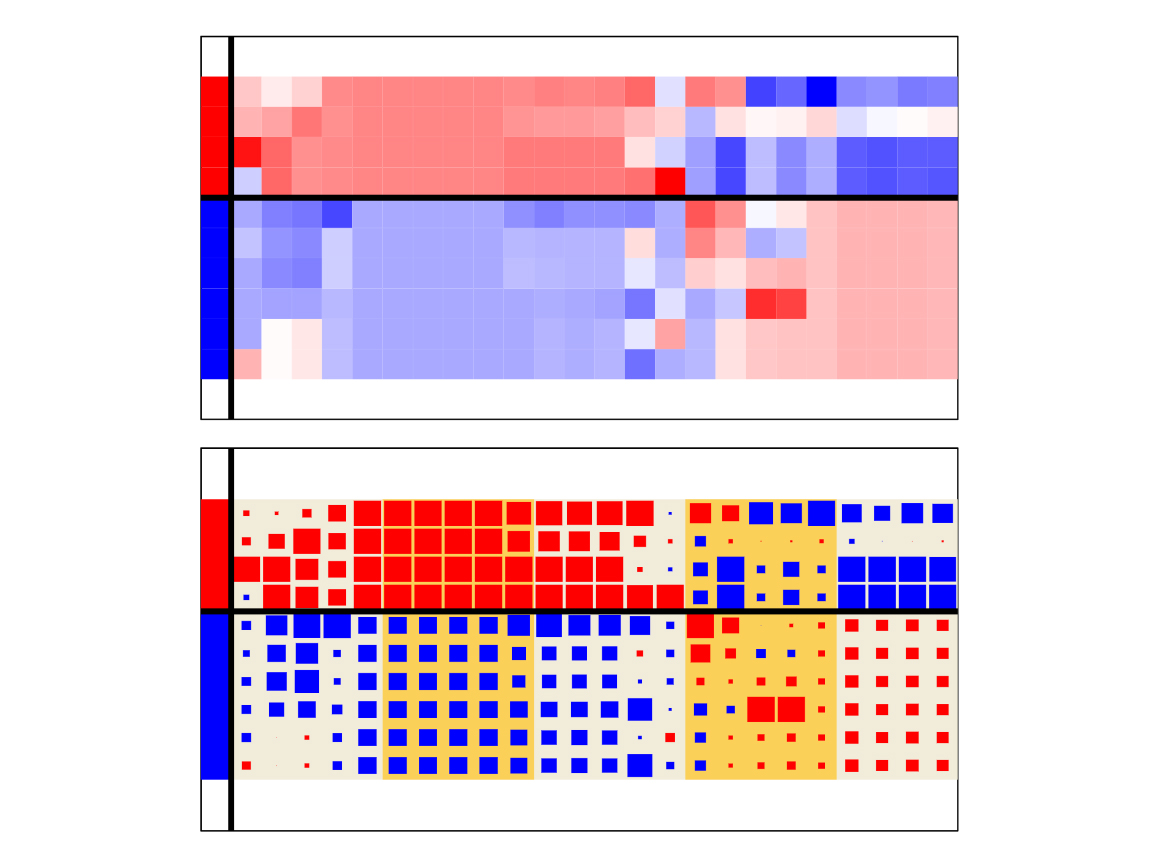
\includegraphics[width=1\linewidth]{ch-visualizer/figures/heatmap}
		\caption[Heatmap versus association navigator]{Heatmap versus 
		association navigator example.}
		\label{fig:visualizer:heatmap}
	\end{center}
\end{figure}

\subsection{System output}
\label{sec:visualizer:plotgeneration:output}

There are three options at the end of stage 2. Two of them are concrete outputs 
that may be easily used in an analyst's final report, and the third is a 
refinement of the active learning component in stage 1.

\tablespacing
\begin{itemize}
	\item \textbf{Automatic plot generation:} The VS compiles a selection of 
	the most interesting and non-interesting plots along with their 
	associated transformation variables.
	\item \textbf{Graph comparison:} The VS accepts a numeric graph (For 
	example, a correlation graph $G^{\text{num}}$ generated with numerical 
	correlation 
	coefficients as described in Section~\ref{sec:intro:correlation}) and 
	measures the difference between the numeric graph $G^{\text{num}}$ and 
	visual graph $G$ (the active learning output). 
	Details on different graph comparison methods may be found in 
	Chapter~\ref{ch:gc}.
	\item \textbf{Line-up test:} In the event that the classifier is not a 
	satisfactory representation of the analyst's interests, the VS may utilize 
	line-up tests to help determine where to query from further. For more 
	details on this methodology, see Section~\ref{sec:futurework:lineup}.
\end{itemize}
\bodyspacing

With the focus on correlation graphs in this work, graph comparison is the most 
useful output from the visualization system. As such, it is one of our primary 
VS focuses. The next section provides a roadmap for the rest of this work, 
which goes into detail on two aspects of the VS. 